%%%%%%%%%%%%%%%%%%%%%%%%%%%%%%%%%%%%%%%%%%%%%%%%%%%%%%%%%%%%%%
% Background
%%%%%%%%%%%%%%%%%%%%%%%%%%%%%%%%%%%%%%%%%%%%%%%%%%%%%%%%%%%%%%
\documentclass[../paper.tex]{subfiles}
\begin{document}
    Consider a mesh consisting of eight cells, as illustrated in \Cref{fig:mesh_example}.
    If data exchange occurs only between adjacent cells, the mesh can be represented as a dependency
    graph, shown in \Cref{fig:graph_example}.
    To partition the mesh into two domains suitable for parallel processing, the objective
    is to divide it into two submeshes of equal size while
    minimizing the number of edges connecting them.
    This corresponds to partitioning the original graph into two complementary 
    subgraphs of equal number of vertices and with a minimum number of interconnecting edges.
    % In other words, the graph is divided into two balanced subsets by cutting the minimal
    % number of edges.
    
    \begin{figure}[h!]
        \centering
        \begin{subfigure}[b]{0.23\textwidth}
            \centering
            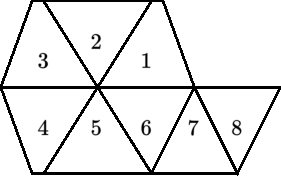
\includegraphics[width=\textwidth]{images/mesh.drawio.svg.pdf}
            \caption{}
            \label{fig:mesh_example}
        \end{subfigure}
        \hfill
        \begin{subfigure}[b]{0.23\textwidth}
            \centering
            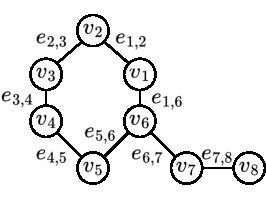
\includegraphics[width=\textwidth]{images/graph.drawio.svg.pdf}
            \caption{}
            \label{fig:graph_example}
        \end{subfigure}
        \caption{Mesh example consisting of 8 parts (left) and the corresponding
        dependency graph (right).}
        \label{fig:mesh_and_graph}
    \end{figure}
    
    
    However, for this bisection problem, finding an optimal solution is NP-hard, making exact computation intractable for large instances \cite{buluc2015recentadvancesgraphpartitioning}. In the following,
    we formalize the graph partitioning problem and introduce bisection algorithms.
    Here, \textit{bisection} specifically refers partitioning the graph into two sub-graphs.
    A general partitioning into $p = 2^l$ sub-graphs can then
    be obtained recursively by applying these bisection methods iteratively.
    
    Let $G=(\mathcal{V}, \mathcal{E})$ be an undirected graph with a vertex set 
    $\mathcal{V}=\{ v_1, \dots, v_n \}$ where each vertex $v_i$ represents
    an element or entity in the problem domain, and an edge set $\mathcal{E}$
    where each edge $e_{i, j} \in \mathcal{E}$ represents a symmetric relation between
    two distinct vertices $v_i$ and $v_j$, meaning that
    $e_{i, j} \in \mathcal{E}$ implies $e_{j, i} \in \mathcal{E}$, and no self-loops exist, i.e., $e_{i, i} \notin \mathcal{E}$. Graphs satisfying these properties are formally referred to as simple and undirected.
    
    The adjacency matrix $\mathbf{A} \in \mathbb{R}^{n \times n}$ of the graph
    stores the connectivity information among its vertices, where the entry
    $\mathbf{A}_{ij}$ is defined as:
    \begin{equation}
      \mathbf{A}_{ij} =
        \begin{cases}
            a_{ij}, & \text{if } e_{i,j} \in \mathcal{E},\\
            0, & \text{otherwise}.
        \end{cases}
    \end{equation}
    
    Here, $a_{ij}$ represents the weight of the edge $e_{i,j}$, which is a nonnegative real-valued number indicating the strength or capacity of the connection
    between vertices $v_i$ and $v_j$. In unweighted graphs, $a_{ij}$ simplifies to 1 for all connected pairs.
    For the simple undirected graphs considered here,the adjacency matrix is symmetric, satisfying $a_{ij} = a_{ji}$ with a zero diagonal, i.e., $a_{ii} = 0$.
    The degree of a vertex $v_i$, denoted as $d_i = \sum^n_j a_{ij}$, represents the sum of the weights of edges incident to $v_i$. In unweighted graphs, $d_i$ reduces to the number of edges connecting $v_i$, effectively counting its direct
    neighbors. The degree matrix $\mathbf{D} \in \mathbb{R}^{n \times n}$ is defined
    as a diagonal matrix, where the diagonal entries correspond to the degrees of all vertices $d_1, \dots, d_n$.
    
    As an example, for the mesh and the corresponding graph depicted in \Cref{fig:mesh_and_graph}, the adjacency matrix $\mathbf{A}$ and the degree matrix $\mathbf{D}$ are given as follows:
    
    \vspace{5mm}
    
    $ \mathbf{A}=
    \begin{pmatrix}
    \color{lightgray} 0 & 1 & \color{lightgray} 0 & \color{lightgray} 0 & \color{lightgray} 0 & 1 & \color{lightgray} 0 & \color{lightgray} 0 \\
    1 & \color{lightgray} 0 & 1 & \color{lightgray} 0 & \color{lightgray} 0 & \color{lightgray} 0 & \color{lightgray} 0 & \color{lightgray} 0 \\
    \color{lightgray} 0 & 1 & \color{lightgray} 0 & 1 & \color{lightgray} 0 & \color{lightgray} 0 & \color{lightgray} 0 & \color{lightgray} 0 \\
    \color{lightgray} 0 & \color{lightgray} 0 & 1 & \color{lightgray} 0 & 1 & \color{lightgray} 0 & \color{lightgray} 0 & \color{lightgray} 0 \\
    \color{lightgray} 0 & \color{lightgray} 0 & \color{lightgray} 0 & 1 & \color{lightgray} 0 & 1 & \color{lightgray} 0 & \color{lightgray} 0 \\
    1 & \color{lightgray} 0 & \color{lightgray} 0 & \color{lightgray} 0 & 1 & \color{lightgray} 0 & 1 & \color{lightgray} 0 \\
    \color{lightgray} 0 & \color{lightgray} 0 & \color{lightgray} 0 & \color{lightgray} 0 & \color{lightgray} 0 & 1 & \color{lightgray} 0 & 1 \\
    \color{lightgray} 0 & \color{lightgray} 0 & \color{lightgray} 0 & \color{lightgray} 0 & \color{lightgray} 0 & \color{lightgray} 0 & 1 & \color{lightgray} 0 
    \end{pmatrix},
    \mathbf{D}=
    \begin{pmatrix}
    2 & \color{lightgray} 0 & \color{lightgray} 0 & \color{lightgray} 0 & \color{lightgray} 0 & \color{lightgray} 0 & \color{lightgray} 0 & \color{lightgray} 0 \\
    \color{lightgray} 0 & 2 & \color{lightgray} 0 & \color{lightgray} 0 & \color{lightgray} 0 & \color{lightgray} 0 & \color{lightgray} 0 & \color{lightgray} 0 \\
    \color{lightgray} 0 & \color{lightgray} 0 & 2 & \color{lightgray} 0 & \color{lightgray} 0 & \color{lightgray} 0 & \color{lightgray} 0 & \color{lightgray} 0 \\
    \color{lightgray} 0 & \color{lightgray} 0 & \color{lightgray} 0 & 2 & \color{lightgray} 0 & \color{lightgray} 0 & \color{lightgray} 0 & \color{lightgray} 0 \\
    \color{lightgray} 0 & \color{lightgray} 0 & \color{lightgray} 0 & \color{lightgray} 0 & 2 & \color{lightgray} 0 & \color{lightgray} 0 & \color{lightgray} 0 \\
    \color{lightgray} 0 & \color{lightgray} 0 & \color{lightgray} 0 & \color{lightgray} 0 & \color{lightgray} 0 & 3 & \color{lightgray} 0 & \color{lightgray} 0 \\
    \color{lightgray} 0 & \color{lightgray} 0 & \color{lightgray} 0 & \color{lightgray} 0 & \color{lightgray} 0 & \color{lightgray} 0 & 2 & \color{lightgray} 0 \\
    \color{lightgray} 0 & \color{lightgray} 0 & \color{lightgray} 0 & \color{lightgray} 0 & \color{lightgray} 0 & \color{lightgray} 0 & \color{lightgray} 0 & 1 
    \end{pmatrix}
    $
    
    \vspace{5mm}
    
    We refer the reader to \cite{doi:https://doi.org/10.1002/9781118601181.ch1} for a detailed overview of commonly used matrices and objectives functions in graph partitioning.
\end{document}